\documentclass[10pt]{beamer}
%\usepackage[sfdefault,light]{FiraSans}
%\usepackage{FiraSans}
%\usepackage{FiraMono}
\usetheme{metropolis}

\usepackage{xspace}
\usepackage{tikz}
\usepackage{amsmath}
\usepackage{pdfpages}
\usepackage{graphics}

\usetikzlibrary{shapes,arrows,positioning,decorations.markings,matrix,fit}
\tikzstyle{line} = [draw,line width=.7pt,fill=none]
\tikzstyle{node} = [draw,circle,minimum width=2em]
\tikzstyle{leaf} = [draw,rectangle,minimum width=2em,minimum height=2em]


\newcommand{\trib}{{\small\raisebox{.75pt}{$\triangleright$}}\xspace}
\newcommand{\tribb}{{\small\raisebox{.75pt}{$\blacktriangleright$}}\xspace}
\newcommand{\tribo}{{\small\raisebox{.75pt}{\textcolor{mLightBrown}{$\blacktriangleright$}}}}

\newcommand{\indtrib}{\hspace*{1em}\trib}
\newcommand{\indtribb}{\hspace*{1em}\tribb}

\definecolor{mBlue}{RGB}{4,110,152}
\definecolor{mGreen}{RGB}{115,180,85}
\definecolor{mRed}{RGB}{205,90,80}
\definecolor{mYellow}{RGB}{230,195,35}
\definecolor{mOrange}{HTML}{EB811B}
\definecolor{mGrey}{RGB}{125,130,140}

\newcommand{\red}[1]{\textcolor{mRed}{#1\xspace}}
\newcommand{\orange}[1]{\textcolor{mLightBrown}{#1}}
\newcommand{\green}[1]{\textcolor{mGreen}{#1\xspace}}
\newcommand{\blue}[1]{\textcolor{mBlue}{#1\xspace}}
\newcommand{\gray}[1]{\textcolor{mGrey}{#1\xspace}}

\newcommand{\akey}[1]{\texttt{#1}\xspace}

\newcommand{\orangea}{\ensuremath{\textcolor{mLightBrown}{\longrightarrow}}\xspace}

\usetikzlibrary{shapes,arrows,positioning,decorations.markings,matrix,fit}
\tikzstyle{line} = [draw, -latex',line width=.7pt,fill=none]
\pgfdeclarelayer{background}
\pgfdeclarelayer{foreground}
\pgfsetlayers{background,main,foreground}

\setbeamertemplate{itemize subitem}{$\circ$}

\title{SMT-COMP 2019\\[2ex]
{\normalsize 14th International
Satisfiability Modulo Theories Competition}}

\author{
  Liana Hadarean \and
  Antti Hyv\"{a}rinen \and
  \underline{Aina Niemetz} \and
  Giles Reger
}

\institute{}

\date{
  \vspace{10ex}
  SMT Workshop, July 7-8, 2019, Lisbon, Portugal
}

\begin{document}
  \maketitle

  \begin{frame}{SMT-COMP}
    \begin{itemize}
      \setbeamertemplate{itemize items}{\orangea}
      \item annual competition for \orange{SMT solvers}
      \item on (a selection of) benchmarks from \orange{SMT-LIB}
    \end{itemize}
    \vspace{1ex}
    \begin{itemize}
      \item first held in \orange{2005}
      \item \orange{2013}: evaluation instead of competition
      \item since \orange{2014}: hosted by StarExec
    \end{itemize}
    \vspace{1ex}
    \textbf{Goals}
    {\vspace{-1ex}\small
    \begin{itemize}
      \setbeamertemplate{itemize items}{$\circ$}
      \item encourage \orange{scientific advances} in SMT solvers
      \item stimulate community to explore \orange{shared challenges}
      \item promote \orange{tools} and their usage
      \item engage and include \orange{new members} of the community
      \item support the \orange{SMT-LIB} project to promote and develop the
        SMT-LIB format and collect relevant benchmarks
    \end{itemize}
    }
  \end{frame}


  \begin{frame}{Participants}
    \textbf{SMT solver:} determine (un)satisfiability 
    of benchmarks from SMT-LIB
    {\small
    \begin{itemize}
      \item \textbf{SMT Solvers} in the `classical' sense
      \item \textbf{Wrapper Tools:} call one or more other SMT solvers
      \item \textbf{Derived Tools:} based on and extends another SMT solver
      \item \textbf{Automated Theorem Provers} (e.g., Vampire)
    \end{itemize}
    }
    \vspace{2ex}
    \begin{itemize}
      \setbeamertemplate{itemize items}{\orangea}
      \item \orange{New} system description mandatory 
      \item \orange{New} naming convention for derived tools
    \end{itemize}
  \end{frame}

  \begin{frame}{Tracks}
    \begin{itemize}
      \item \textbf{Single Query Track} (previously: Main Track)
        \begin{itemize}
          \item one \textbf{single} \akey{check-sat} command,
            no \akey{push}/\akey{pop} commands
          \item \orange{New} \textbf{remove} benchmarks solved by all solvers 
            in 2018 in $\leq 1s$
          \item \orange{New} \textbf{selection} of benchmarks
          \item \orange{New} \textbf{time limit:} 2400s (40 min)
        \end{itemize}
      \vspace{4ex}
      \item \textbf{Incremental Track} (previously: Application Track)
        \begin{itemize}
          \item \textbf{multiple} \akey{check-sat} and \akey{push}/\akey{pop} commands
          \item solvers are executed on benchmarks via \textbf{trace executor}
          \item \orange{New} \textbf{selection} of benchmarks
          \item \orange{New} \textbf{keep} benchmarks with first \akey{check-sat}
            status \akey{unknown}
          \item \orange{New} execute solver \textbf{beyond} first status
            \akey{unknown} \akey{check-sat} call
          \item \textbf{time limit:} 2400s (40 min)
        \end{itemize}
    \end{itemize}
  \end{frame}

  \begin{frame}{Tracks}
    \begin{itemize}
      \item \textbf{Unsat Core Track}
        \begin{itemize}
          \item one \textbf{single} \akey{check-sat} command,
                \textbf{multiple} \akey{assert} commands
          \item benchmarks with \textbf{status \akey{unsat}}
          \item extract \textbf{unsat core} as set of top-level assertions
          \item \orange{New} \textbf{remove} benchmarks with a single \akey{assert} command
          \item \orange{New} \textbf{selection} of benchmarks
          \item \textbf{time limit:} 2400s (40 min)
        \end{itemize}
    \end{itemize}
  \end{frame}

  \begin{frame}{Tracks}
    \begin{itemize}
      \item \orange{New:} \textbf{Challenge Track}
        \begin{itemize}
          \item two subtracks: \orange{non-incremental} and \orange{incremental}
          \item benchmarks that were \textbf{nominated} by their submitters for
            this track
          \item \textbf{time limit:} 43200s (12 hours)
        \end{itemize}
      \vspace{4ex}
      \item \orange{New:} \textbf{Model Validation Track} (\orange{experimental})
        \begin{itemize}
          \item one \textbf{single} \akey{check-sat} command,
          \item \textbf{selection} of benchmarks with \textbf{status \akey{sat}}
          \item produce full, correct, well-formed
            \textbf{model} in SMT-LIB format
          \item \textbf{only} for division QF\_BV
          \item \textbf{time limit:} 2400s (40 min)
        \end{itemize}
      \end{itemize}
  \end{frame}

  \begin{frame}{Divisions}
    \begin{itemize}
      \setbeamertemplate{itemize items}{\orangea}
      \item \textbf{Tracks} are split into divisions
      \item \textbf{Divisions} correspond to \orange{logics} in SMT-LIB
    \end{itemize}
    \begin{itemize}
      \item solvers are submitted to divisions in a track
      \item \textbf{winners} are declared
        \begin{itemize}
          \item per division and track
          \item with respect to different scoring schemes per track
        \end{itemize}
      \vspace{1ex}
      \item \orange{New} do not run \textbf{non-competitive} divisions
    \end{itemize}
  \end{frame}

  \begin{frame}{Benchmark Selection}
    \begin{itemize}
      \item \orange{2015-2018}: \textbf{all} eligible benchmarks in a division
        \begin{itemize}
          \setbeamertemplate{itemize items}{$\longrightarrow$}
          \item results more predictable
          \item more of an evaluation than a competition
          \item Main Track (2018):
            \begin{itemize}
              \setbeamertemplate{itemize items}{$\circ$}
              \item 78\% solved by all participating solvers
              \item 71\% solved in $\leq 1s$
              \item in 7 out of 46 divisions $> 99\%$ solved by all solvers
            \end{itemize}
        \end{itemize}
      \vspace{1ex}
      \item \orange{New} alternative benchmark selection
        \begin{itemize}
          \item \textbf{remove} easy/uninteresting benchmarks
            \begin{itemize}
              \item SQ:
                all benchmarks solved by all solvers in $\leq 1 s$ in 2018
              \item UC: all benchmarks with only a single assertion
            \end{itemize}

          \item \textbf{cap} number of instances in a division
            \begin{itemize}
              \item $n \leq 300$: all instances
              \item $300 < n \leq 600$: 300 instances
              \item $n > 600$: 50\% of the logic
            \end{itemize}

          \item guarantee inclusion of \textbf{new} benchmarks
            (at least one per family)

          \item select benchmarks randomly using a uniform distribution
        \end{itemize}
    \end{itemize}
  \end{frame}

  \begin{frame}{Single Query and Unsat Core Track Scoring}
    \begin{itemize}
      \item \orange{2016-2018}:
        \textbf{weighted} with respect to benchmark family size
        \begin{itemize}
          \setbeamertemplate{itemize items}{$\longrightarrow$}
          \item \textbf{goal:} de-emphasize large benchmark families
          \item fairly complicated, not necessarily intuitive
          \item complicates comparing paper and competition results
        \end{itemize}
      \vspace{2ex}
      \item \textbf{Competition report} for 2015-2018 (under review):
        \begin{itemize}
          \setbeamertemplate{itemize items}{\orangea}
          \item families \textbf{no significant impact} on the (weighted)
            scores
            \begin{itemize}
              \setbeamertemplate{itemize items}{$\circ$}
              \item problems with scoring script (2016-2018)
              \item incorrect interpretation of benchmark family 
              \item \textbf{after fix:} only one change
              (2017 AUFNIRA: CVC4 over Vampire)
            \end{itemize}
          \item \textbf{unweighted:} only 7 out of 139 winners in
            2016-2018 change
      \end{itemize}
      \vspace{2ex}
      \item \orange{New} drop weighted scoring, use \textbf{unweighted} scheme
        from 2015
    \end{itemize}
  \end{frame}

  \begin{frame}{Scores}
    \begin{itemize}
      \item \textbf{Single Query, Challenge (non-incremental):}\\
        number of correctly solved instances
      \vspace{1ex}
      \item \textbf{Incremental, Challenge (incremental):}\\
        number of correctly solved \akey{check-sat} calls
      \vspace{1ex}
      \item \textbf{Unsat Core:}\\
        reduction in terms of top-level assertions
      \vspace{1ex}
      \item \textbf{Model Validation:}\\
        number of correctly solved instances with validated models
    \end{itemize}
  \end{frame}

  \begin{frame}{Scores}
    \begin{itemize}
      \item \textbf{sequential score} (SQ, CHSQ, UC, MV)\\
        time limit applied to CPU time
      \vspace{1ex}
      \item \textbf{parallel score} (all)\\
        time limit applied to wall-clock time
      \vspace{1ex}
      \item \orange{New} \textbf{sat score} (SQ, CHSQ)\\
        parallel score for satisfiable instances
      \vspace{1ex}
      \item \orange{New} \textbf{unsat score} (SQ, CHSQ)\\
        parallel score for unsatisfiable instances
      \vspace{1ex}
      \item \orange{New} \textbf{24s score} (SQ, CHSQ)\\
        parallel score for time limit of 24s
    \end{itemize}
  \end{frame}

  \begin{frame}{Competition-Wide Recognitions}
    \begin{itemize}
      \item \orange{2014-2018}:
        \begin{itemize}
          \setbeamertemplate{itemize items}{$\circ$}
          \item \textbf{competition-wide scores} as weighted sum of division
            scores
          \item emphasis on number of entered divisions
        \end{itemize}
      \vspace{1ex}
    \item \orange{New} replace with \textbf{two new competition-wide
      rankings}
      \begin{itemize}
        \setbeamertemplate{itemize items}{$\longrightarrow$}
        \item focus on measures that make sense to compare between divisions
        \item for all scores in a track
        \setbeamertemplate{itemize items}{$\circ$}
      \end{itemize}
      \vspace{1ex}
      \item \orange{\textbf{biggest lead}}
        \begin{itemize}
          \item in terms of \textbf{score} over the solver in the second place
          \item \textbf{tie:} ranked by biggest lead in CPU/wall-clock time
        \end{itemize}
      \vspace{1ex}
        \item \orange{\textbf{largest contribution}}
          \begin{itemize}
            \item ranked by contribution to \textbf{virtual best solver}
              in terms of \textbf{score}
            \item \textbf{tie:} ranked by largest contribution in terms of
              CPU/wall-clock time
          \end{itemize}
    \end{itemize}
  \end{frame}

  \begin{frame}{Competition Overview}

    {\footnotesize
      \begin{tabular}{r|r@{\hspace{.75em}}r|r@{\hspace{.75em}}r|r@{\hspace{.75em}}r@{\hspace{.75em}}r}
        & \multicolumn{2}{c}{\textbf{Solvers}}
        & \multicolumn{2}{|c}{\textbf{Divisions}}
        & \multicolumn{3}{|c}{\textbf{Benchmarks}} \\
        \textbf{Track}
        & \textbf{Total}
        & \textbf{C/NC}
        & \textbf{Total}
        & \textbf{C/NC/Exp}
        & \textbf{C}
        & \textbf{Selected}
        & \textbf{Total}
        \\
        \hline
        SQ    & 51 (\orange{+27}) &  37/\gray{14} & 57 (\orange{+7}) & 49/\gray{6}/2 & 64156 & 89817 & 327041 \\
        Inc   & 22 (\orange{+16}) &  14/\gray{8}  & 29 (\orange{+8}) & 24/\gray{5}/0 &  6835 &  7567 & 14030 \\
        CHSQ  & 21 (\orange{+21}) &  15/\gray{6}  &  3 (\orange{+3}) &  3/\gray{0}/0 &    29 &    29 & 29 \\
        CHInc & 12 (\orange{+12}) &   7/\gray{5}  &  3 (\orange{+3}) &  3/\gray{0}/0 &    22 &    22 & 22 \\
        UC    & 14 (\orange{+9})  &   8/\gray{6}  & 38 (\orange{-6}) & 33/\gray{5}/0 & 29808 & 44341 & 136012\\
        MV    & 10 (\orange{+10}) &  10/\gray{0}  &  1 (\orange{+1}) &  1/\gray{0}/0 &  7191 &  7191 & 14382 \\
      \end{tabular}
      \begin{center}
        C \ldots Competitive
        \hspace{1.5em}NC \ldots Non-Competitive
        \hspace{1.5em}Exp \ldots Experimental\\
      \end{center}
    }

    \vfill
    \textbf{Teams}: 23 (\alert{+6})\\
    \textbf{StarExec Stats}: 21.4 years CPU time; 1,022,802 job pairs
    \vfill
  \end{frame}

  \begin{frame}{Non-Competitive Solvers}
    \textbf{Total:} \textbf{\orange{14}} (SQ), \textbf{\orange{8}} (Inc),
    \textbf{\orange{6}} (CHSQ),
    \textbf{\orange{5}} (CHINC), \textbf{\orange{6}} (UC)
    \begin{itemize}
      \item submitted by \textbf{organizers}
        \begin{itemize}
          \item Z3 4.8.4
          \item best solvers 2018 (SQ: 9, Inc: 5, CHSQ: 3, CHINC: 3, UC: 5)
        \end{itemize}
      \vspace{1ex}
      \item submitted by \textbf{participants}
        \begin{itemize}
          \item 2 derived tools (Boolector-ReasonLS, CVC4-SymBreak)
          \item 3 fixed solver versions (1 x CVC4, 2 x STP)
        \end{itemize}
    \end{itemize}
  \end{frame}

\begin{frame}{Solver Presentations}
  \begin{center}
    Boolector, COLIBRI, CVC4, MathSAT, OpenSMT, SPASS-SATT,
    Vampire,
    VeriT
    Yices
  \end{center}
\end{frame}

{
  \setbeamercolor{background canvas}{bg=}
  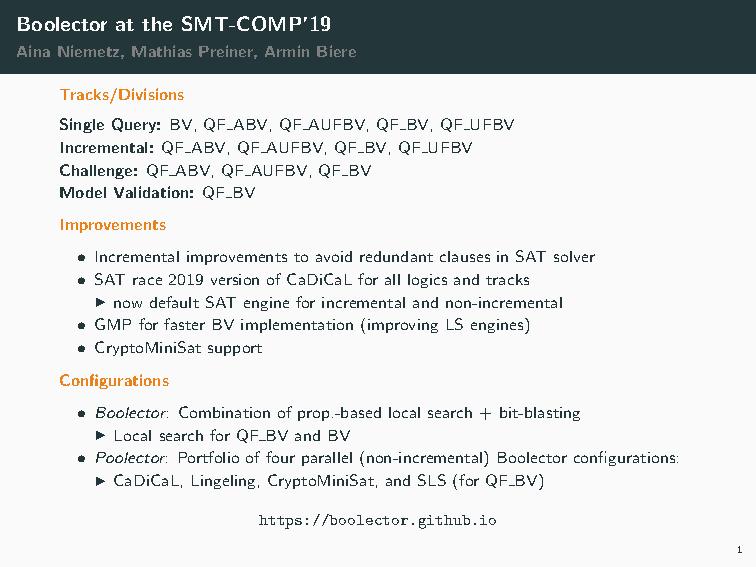
\includepdf[pages=1-]{solvers/boolector.pdf}
  
\includepdf[pages=1-2]{solvers/colibri.pdf}
  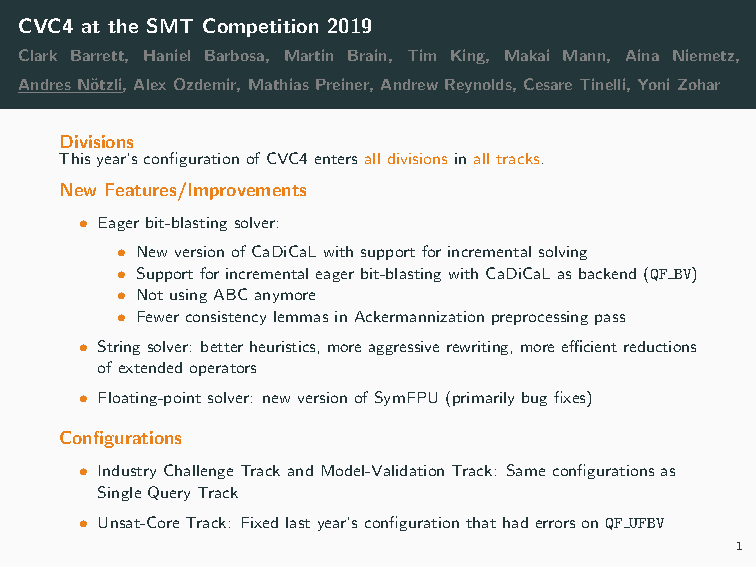
\includepdf[pages=1-]{solvers/cvc4.pdf}
  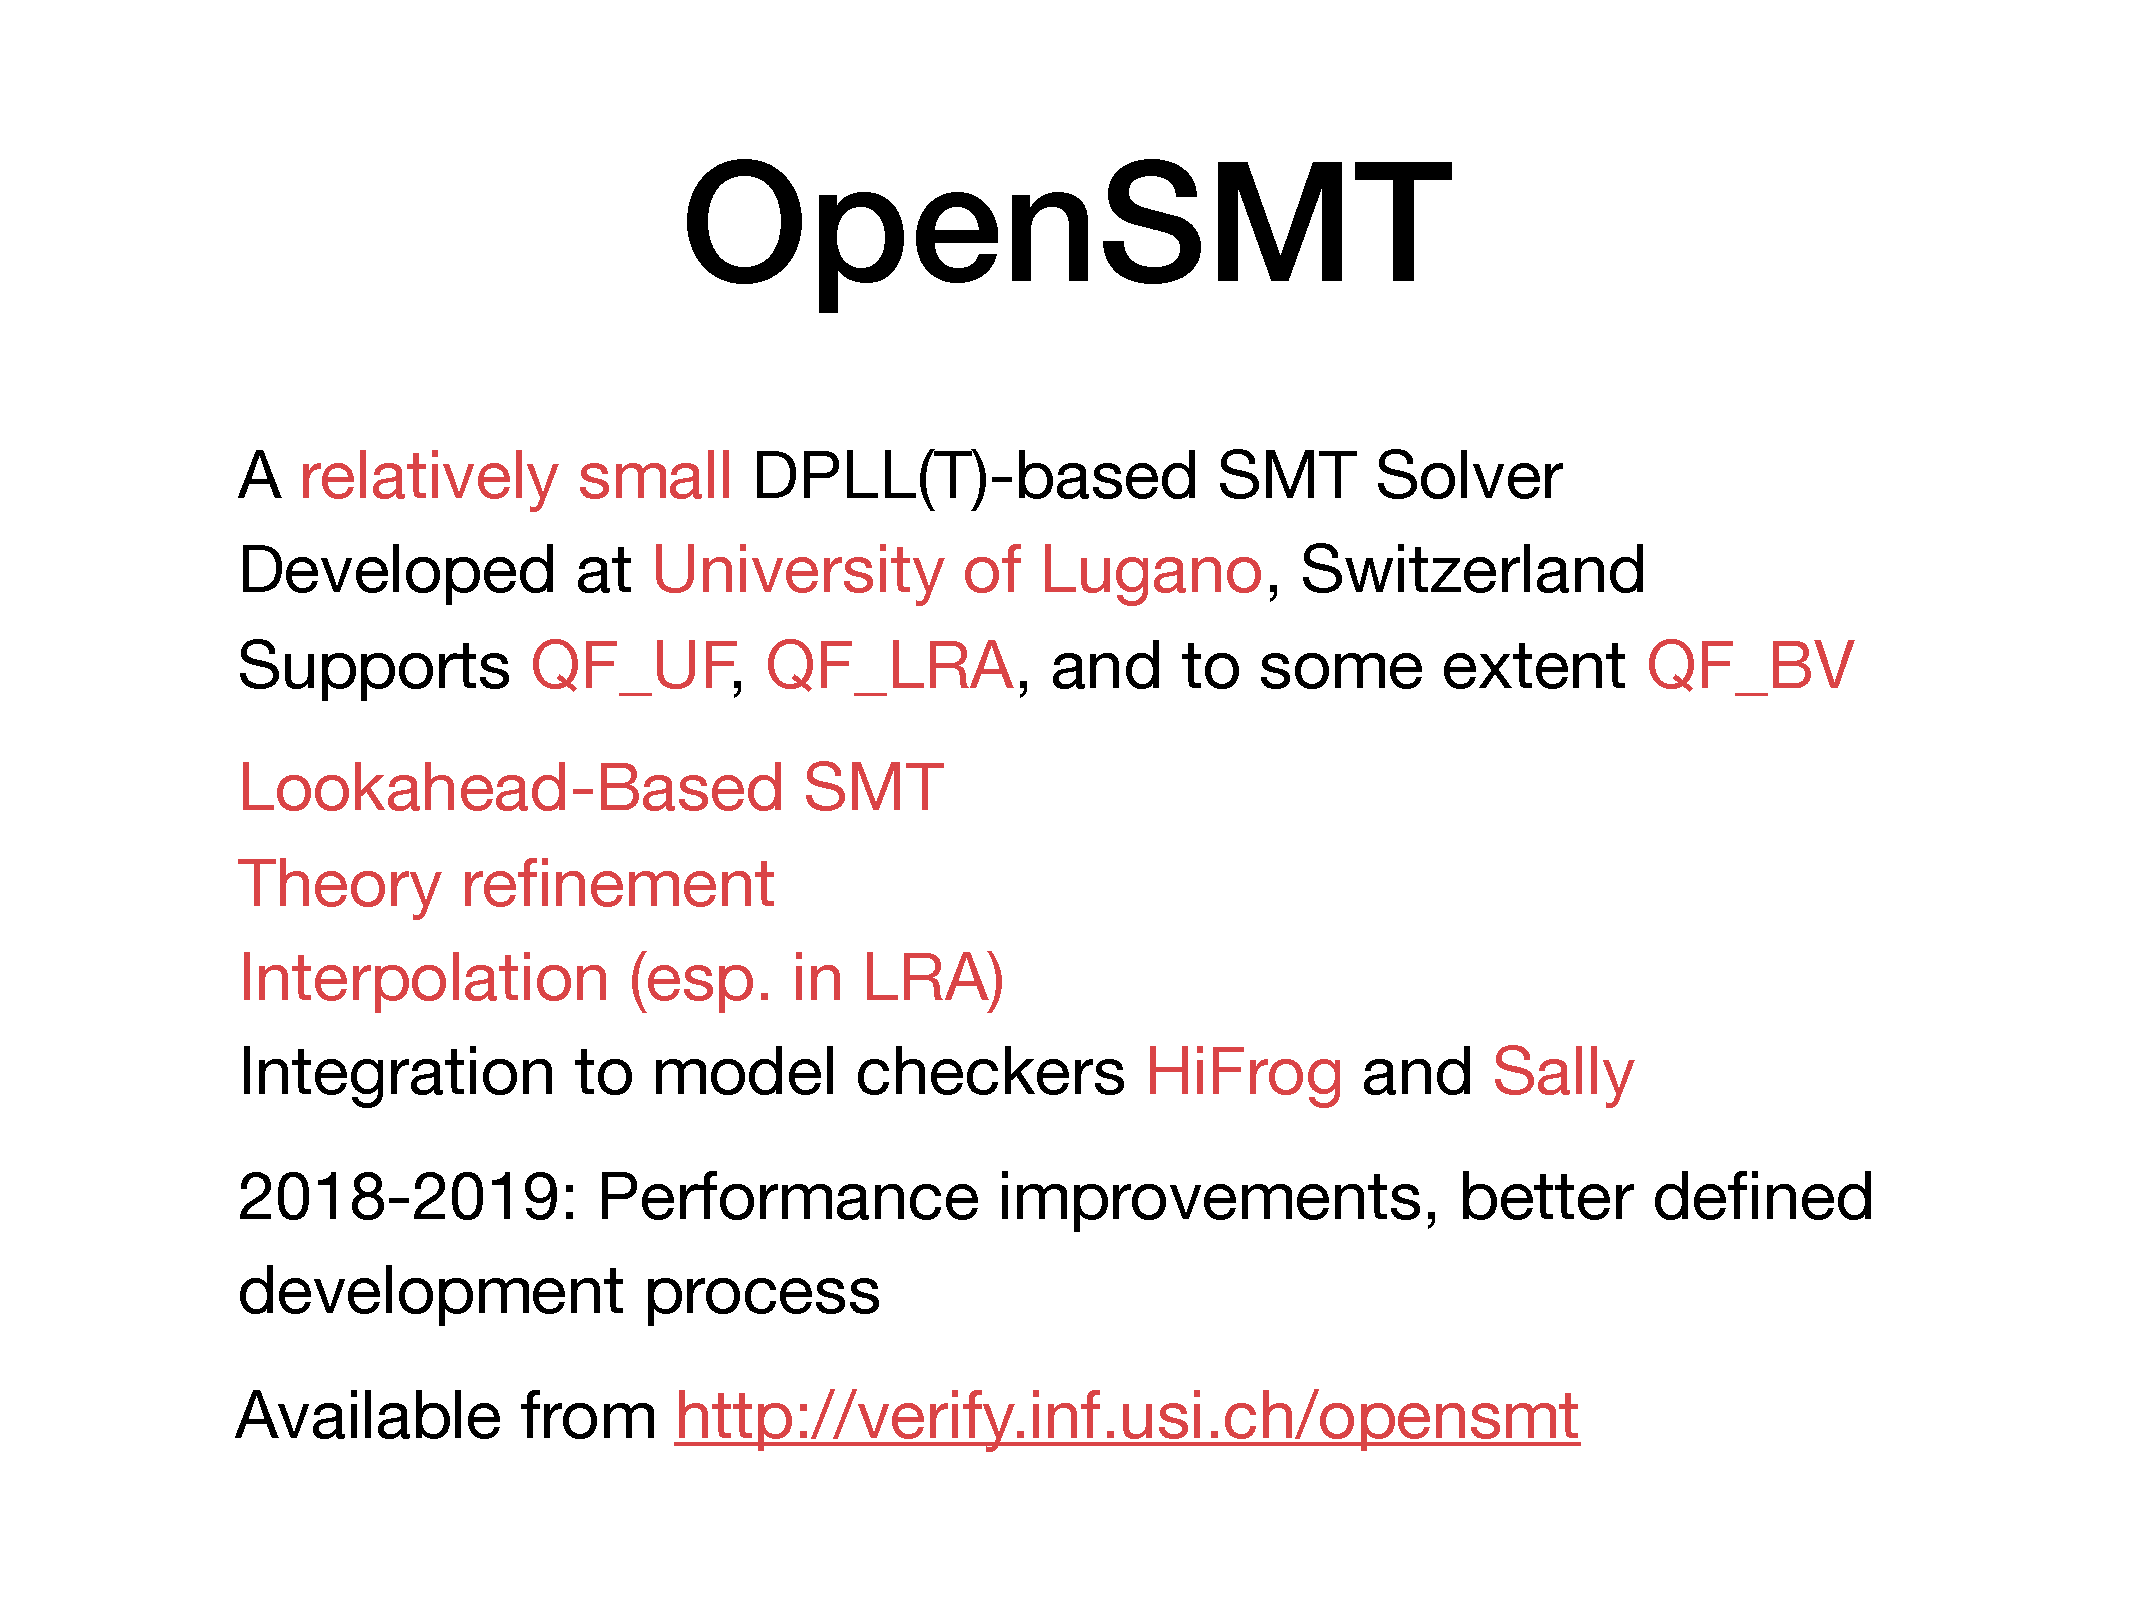
\includepdf[pages=1-]{solvers/opensmt.pdf}
  
\includepdf[pages=1-]{solvers/SPASS-SATT2.pdf}
  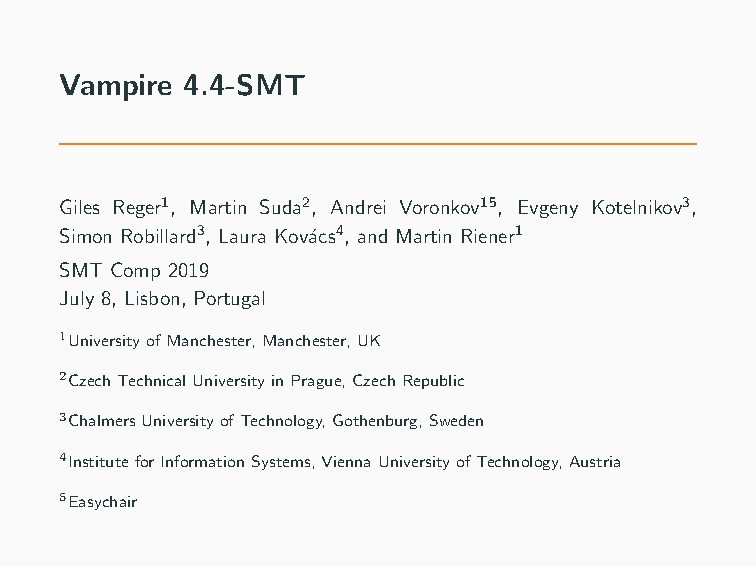
\includepdf[pages=1-]{solvers/vampire.pdf}
  
\includepdf[pages=1-]{solvers/verit.pdf}
  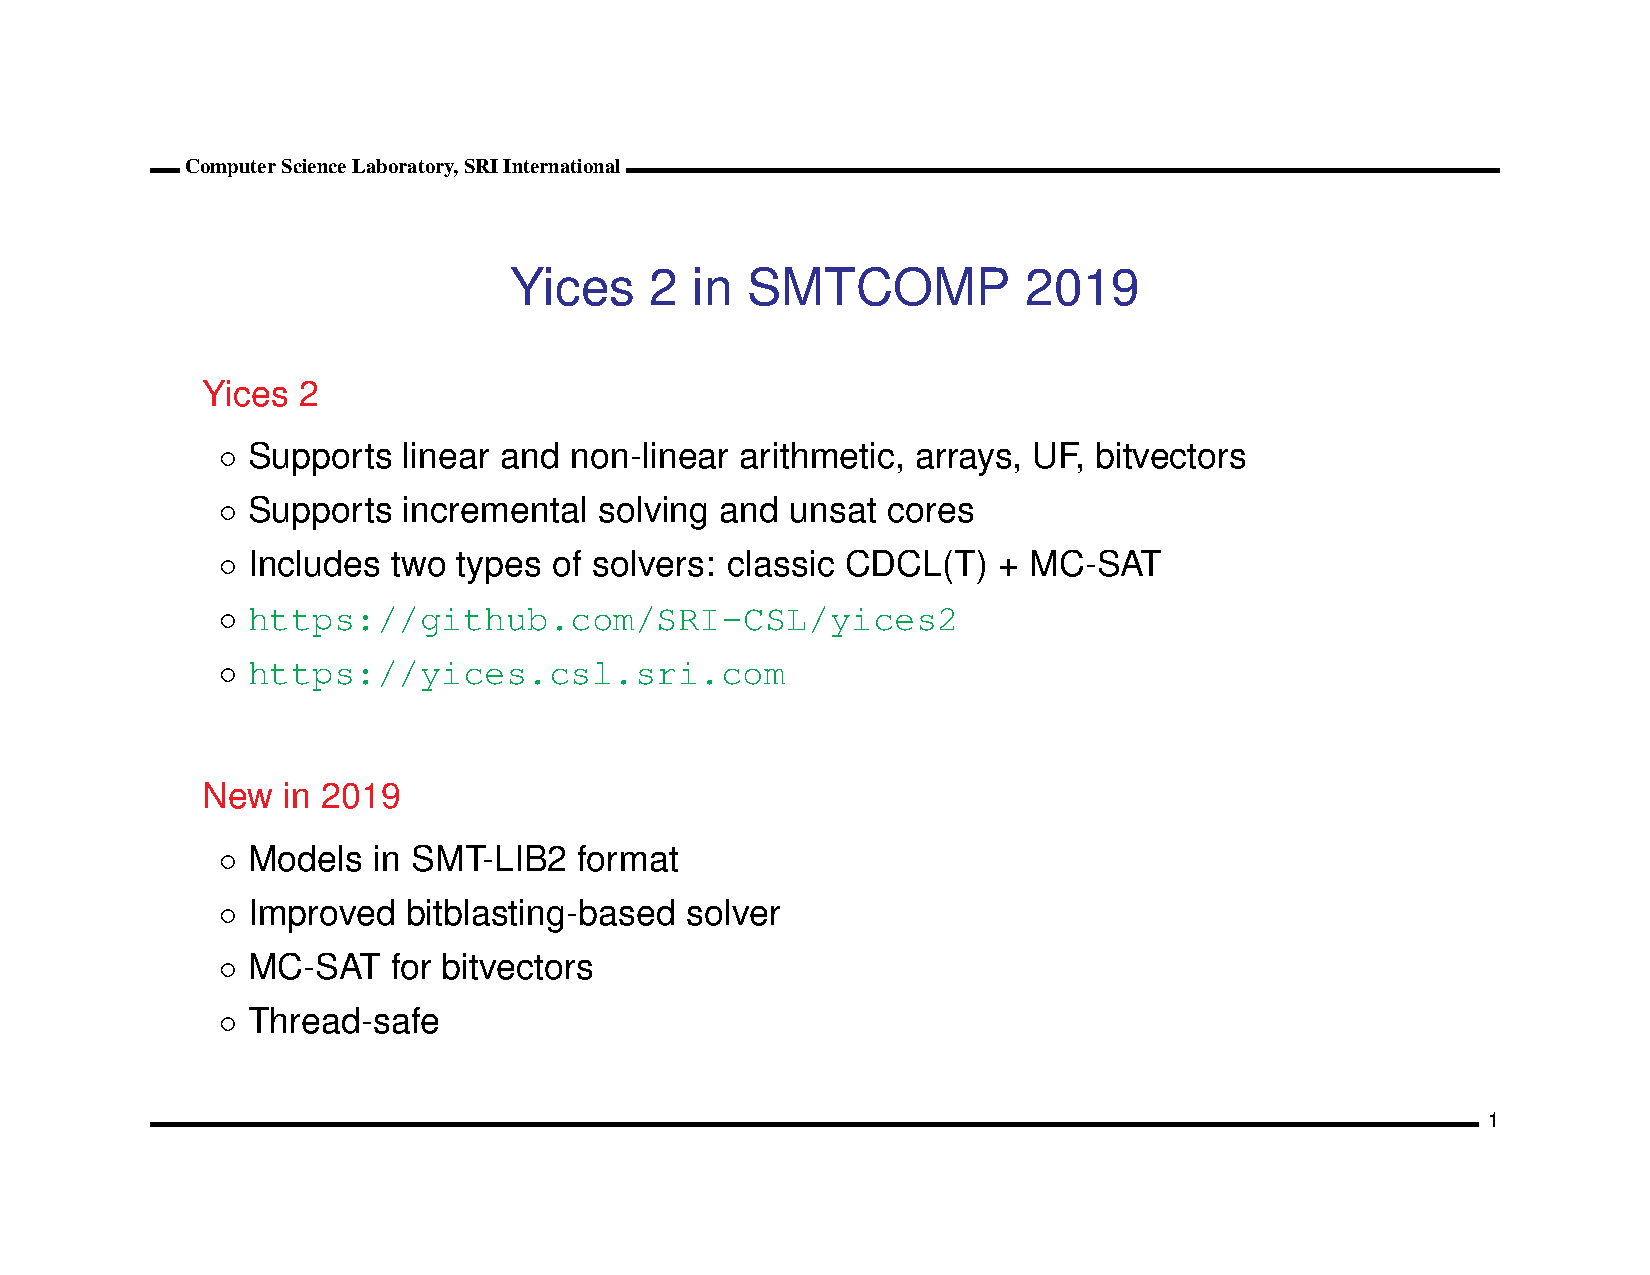
\includepdf[pages=1-]{solvers/yices.pdf}
  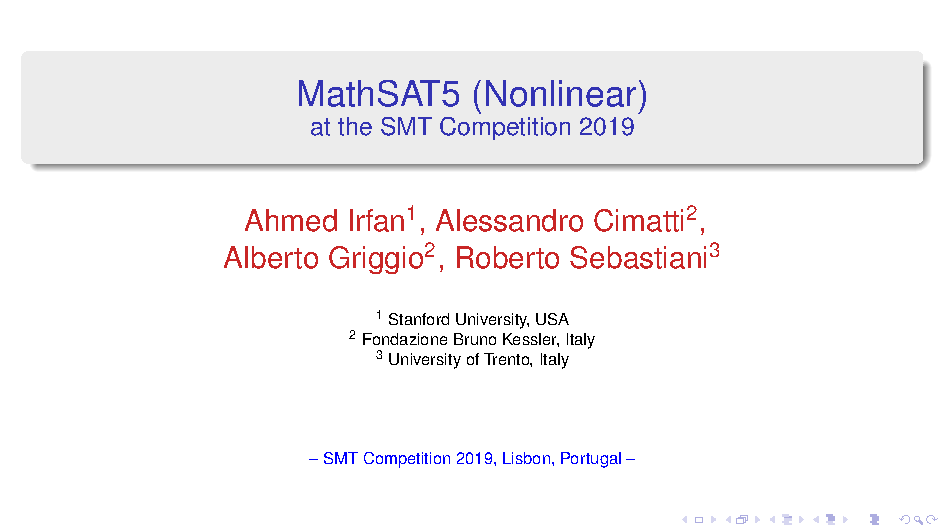
\includepdf[pages=1]{solvers/mathsat.pdf}
  \includepdf[pages=4]{solvers/mathsat.pdf}
}

  \begin{frame}{Results}
    \begin{center}
    \resizebox{.9\textwidth}{!}{
      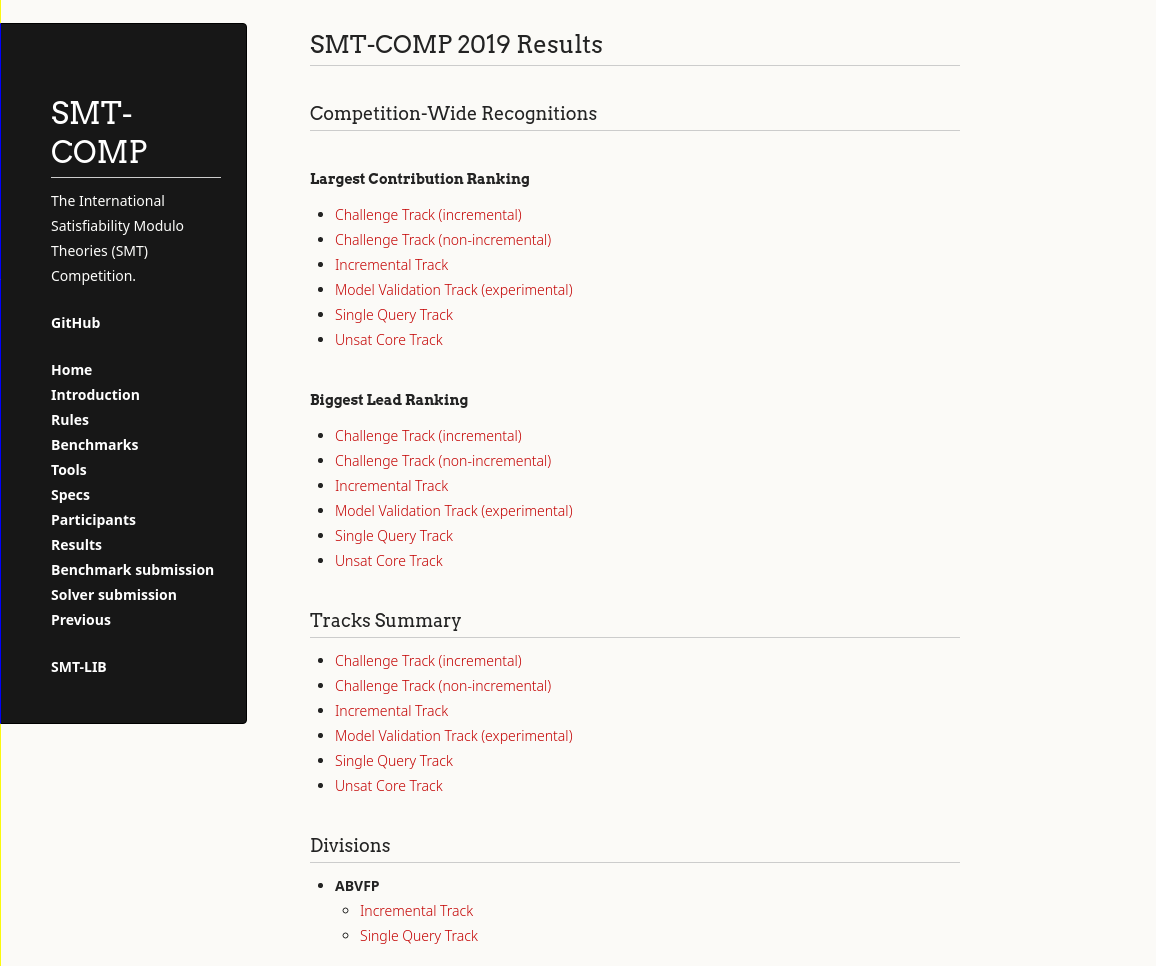
\includegraphics{results.png}
    }
    \end{center}
  \end{frame}

  \begin{frame}{Competition-Wide Recognitions}
    \begin{center}
      {\Huge Trophies}
    \end{center}
  \end{frame}

  \begin{frame}{Trophies: Largest Contribution}

    \begin{tabular}{rrr}
      \hline
      \textbf{Single Query}
      & \textbf{1\textsuperscript{st} Place}
      & \textbf{2\textsuperscript{nd} Place} \\
      seq   & \textbf{\orange{CVC4}} (QF\_NIA)  & \textbf{Vampire} (UF) \\
      par   & \textbf{\orange{CVC4}} (QF\_NIA)  & \textbf{Vampire} (UF) \\
      sat   & \textbf{\orange{Par4}} (AUFLIRA)  & \textbf{SMTInterpol} (UFLIA) \\
      unsat & \textbf{\orange{Par4}} (UFNIA)    & \textbf{Vampire} (UF) \\
      24s   & \textbf{\orange{Vampire}} (UF)    & \textbf{Par4} (UFNIA) \\
      \hline
      \hline

      \textbf{Incremental}
      & \textbf{1\textsuperscript{st} Place}
      & \textbf{2\textsuperscript{nd} Place} \\
      par &  \textbf{\orange{CVC4}} (UFLRA) & \textbf{Boolector} (QF\_BV) \\
      \hline
      \hline

      \textbf{Unsat Core}
      & \textbf{1\textsuperscript{st} Place}
      & \textbf{2\textsuperscript{nd} Place} \\
      seq & \textbf{\orange{CVC4}} (AUFLIRA) & \textbf{MathSAT} (QF\_NIA) \\
      par & \textbf{\orange{CVC4}} (AUFLIRA) & \textbf{MathSAT} (QF\_NIA) \\
      \hline
      \hline

      \textbf{Challenge}
      & \textbf{1\textsuperscript{st} Place}
      & \textbf{2\textsuperscript{nd} Place} \\
      par & \textbf{\orange{Yices}} (QF\_AUFBV) & \textbf{Boolector} (QF\_ABV) \\
      \hline

    \end{tabular}
  \end{frame}

  \begin{frame}{Trophies: Biggest Lead}

    \begin{tabular}{rrr}
      \hline
      \textbf{Single Query}
      & \textbf{1\textsuperscript{st} Place}
      & \textbf{2\textsuperscript{nd} Place} \\
      seq   &  \textbf{\orange{CVC4}} (FP)       &  \textbf{Par4} (UFBV) \\
      par   &  \textbf{\orange{CVC4}} (FP)       &  \textbf{Par4} (UFBV) \\
      sat   &  \textbf{\orange{CVC4}} (AUFDTLIA) &  \textbf{Par4} (AUFLIRA) \\
      unsat &  \textbf{\orange{CVC4}} (BVFP)     &  \textbf{SMT-RAT} (QF\_NIRA) \\
      24s   &  \textbf{\orange{CVC4}} (BVFP)     &  \textbf{Par4} (UFBV) \\
      \hline
      \hline

      \textbf{Incremental}
      & \textbf{1\textsuperscript{st} Place}
      & \textbf{2\textsuperscript{nd} Place} \\
      par & \textbf{\orange{CVC4}} (ANIA)  & \textbf{Yices} (QF\_AUFBV) \\
      \hline
      \hline

      \textbf{Unsat Core}
      & \textbf{1\textsuperscript{st} Place}
      & \textbf{2\textsuperscript{nd} Place} \\
      seq & \textbf{\orange{CVC4}} (UFLIA) &  \textbf{Yices} (QF\_AX) \\
      par & \textbf{\orange{CVC4}} (UFLIA) &  \textbf{Yices} (QF\_AX) \\
      \hline
      \hline

      \textbf{Challenge}
      & \textbf{1\textsuperscript{st} Place}
      & \textbf{2\textsuperscript{nd} Place} \\
      par & \textbf{\orange{Yices}} (QF\_AUFBV) & \textbf{Boolector} (QF\_ABV) \\
      \hline
    \end{tabular}
  \end{frame}

  \begin{frame}{Discussion}
    \begin{itemize}
      \item \textbf{time limit}
        \begin{itemize}
          \item increased back to 2400s (from 1200s 2017-2018) in SQ track
          \item only \orange{$-3953$} instances if cut off at \textbf{1200s}
            (sequential score)
          \item \orange{$\sim50\%$} of the timeouts in \textbf{quantified}
            divisions
          \vspace{2ex}
          \setbeamertemplate{itemize items}{\orangea}
          \item run selected challenging benchmarks in the \textbf{challenge track}
          \vspace{1ex}
          \item \textbf{decrease} time limit (maybe even further) for \textbf{other tracks}
          \vspace{1ex}
          \item shorter time limit for \textbf{quantified divisions}?
            \\
            (typically: solved within short time or ``never")
        \end{itemize}
    \end{itemize}
  \end{frame}

  \begin{frame}{Discussion}
    \begin{itemize}
      \item \textbf{divisions}
        \begin{itemize}
          \item size of competitions is getting out of hand
          \item this year we didn't run non-competitive divisions
          \vspace{2ex}
          \setbeamertemplate{itemize items}{\orangea}
          \item \textbf{don't run} if less than 3? 4? competitive participants?
        \end{itemize}
      \vspace{2ex}
      \item \textbf{parallel score}
        \begin{itemize}
          \setbeamertemplate{itemize items}{$\circ$}
          \item StarExec only offers 4 cores per job
          \item not interesting for real parallelism
          \vspace{1ex}
          \setbeamertemplate{itemize items}{\orangea}
          \item \textbf{future plans:} dedicated \textbf{parallel track}
          \item would require to move away from StarExec
        \end{itemize}
      \end{itemize}
  \end{frame}

  \begin{frame}{Discussion}
    \begin{itemize}
      \item \textbf{portfolio wrapper tools}
        \begin{itemize}
          \item wrapper tools allowed to participate without restrictions
          \vspace{1ex}
          \item problems with portfolio
            (not author of the wrapped solvers)
            \begin{itemize}
              \setbeamertemplate{itemize items}{$\rightarrow$}
              \item win with simple script and work of other teams
              \item negative/unfair impact on competition-wide rankings
              \item progress of non-portfolio tools harder to distinguish
            \end{itemize}
          \vspace{1ex}
          \item disallowing wrapper tools entirely is problematic (example: Vampire)
          \vspace{2ex}
          \setbeamertemplate{itemize items}{\orangea}
          \item \textbf{disallow} portfolio with wrapped solvers from other teams?
          \vspace{1ex}
          \item only allow \textbf{non-competitive} submission?
          \vspace{1ex}
          \item at least \textbf{exclude} them from competition-wide recognitions
          \vspace{1ex}
          \item \textbf{similar issues} with SATzilla-style systems
        \end{itemize}
    \end{itemize}
  \end{frame}

  \begin{frame}{Ackknowledgements}
    \begin{itemize}
      \item Mathias Preiner (benchmark selection and scoring scripts)
      \item Aaron Stump (StarExec)
      \item Andres N\"{o}tzli (trace executor extension)
      \item Marco Gario and Andrea Micheli (PySMT)
      \item Martin Riener (certificates/trophies logistics)
    \end{itemize}
  \end{frame}
\end{document}
